\chapter{Resultados}

Na tabela \ref{estadoAtual} pode ser visualizado as Histórias de Usuário, a pontuação e o estado (a fazer, em progresso ou feito) de cada História. \textcolor{red}{Foram implementados 12 pontos do total de 48 pontos estimados. Sendo assim, já foi implementado 25\% dos pontos da ferramenta InvestMVC}.

\begin{table}[H]
\caption{Estado atual da ferramenta InvestMVC}
\begin{center}
    \begin{tabular}{ | c | c | c |}
    \hline
    \textbf{Histórias de Usuário} & \textbf{Pontuação} & \textbf{Estado} \\ \hline

US1 - Agente Correlação Linear & 3 & Feito\\ \hline
US2 - Agente Fibonacci & 3 & Feito \\ \hline
US3 - Agente Mínimos Quadrados & 3 & Feito\\ \hline
US4 -  Agente Tendência & 2 & Feito\\ \hline
US5 - Agente Gestor/Consultor & 2& Feito\\ \hline
US6 - Criar conta de usuário & 2 & Feito\\ \hline
US7 - Acompanhar retorno financeiro & 5 & A fazer\\ \hline
US8 - Criar Experts & 2 & Feito\\ \hline
US9 - Editar Experts & 2 & Feito\\ \hline
US10 - Excluir Experts & 2 & Feito\\ \hline
US11 - Ativar Expert & 1 & Feito\\ \hline
US12 - Desativar Expert & 2 & A fazer \\ \hline
US13 - Método Correlação Linear em linguagem C & 2 & Feito\\ \hline
US14 - Método Fibonacci em linguagem C & 2 & Feito\\ \hline
US15 - Método Mínimos Quadrados em linguagem C & 2 & Feito\\ \hline
US16 - Método Correlação Linear em linguagem Haskell & 2 & Feito\\ \hline
US17 - Método Fibonacci em linguagem Haskell & 2 & Feito\\ \hline
US18 - Método Mínimos Quadrados em linguagem Haskell & 2 & Feito\\ \hline
US19 - Inserir na Base de Conhecimento & 2 & Feito\\ \hline
US20 - Retirar na Base de Conhecimento & 2 & A fazer\\ \hline
US21 - Calcular Critério de Entrada & 3 & Feito\\ \hline
US22 - Realizar Operação no MetaTrader& 1 & A fazer\\ \hline
\end{tabular}
\end{center}
\label{estadoAtual}
\end{table}


\section{Resultados testes unitários}

\subsection{Componente Funcional}

Foram realizados os testes unitários na linguagem haskell utilizando o framework HUnit. O framework não fornece a cobertura de código fonte, mas é possível visualizar a quantidade de casos de teste, quantidade de testes realizados, quantidade de erros e quantidade de falhas. Os resultados dos testes unitários dos métodos de Correlação de Pearson, Fibonacci e Mínimos Quadrados podem ser visualizados na Figura \ref{testeCorrelacaoHaskell}, \ref{testeFibonacciHaskell} e \ref{TesteMinimosHaskell}.

\begin{figure}[H]
\centering
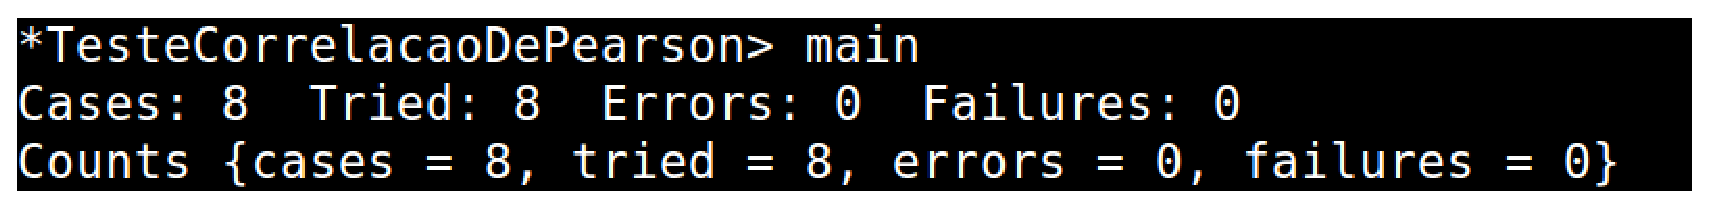
\includegraphics[width=0.9\textwidth]{figuras/testeCorrelacaoHaskell}
\caption{Resultado da Suíte de Teste do Método Correlação Linear}
\label{testeCorrelacaoHaskell}
\end{figure}

\begin{figure}[H]
\centering
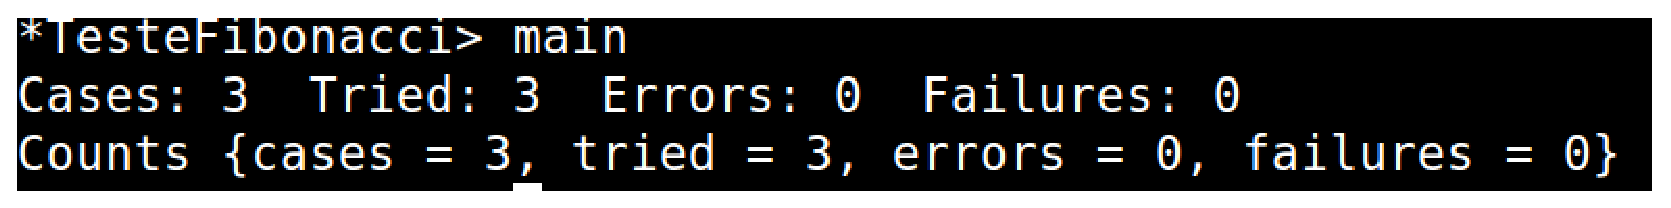
\includegraphics[width=0.9\textwidth]{figuras/testeFibonacciHaskell}
\caption{Resultado da Suíte de Teste do Método de Fibonacci}
\label{testeFibonacciHaskell}
\end{figure}

\begin{figure}[H]
\centering
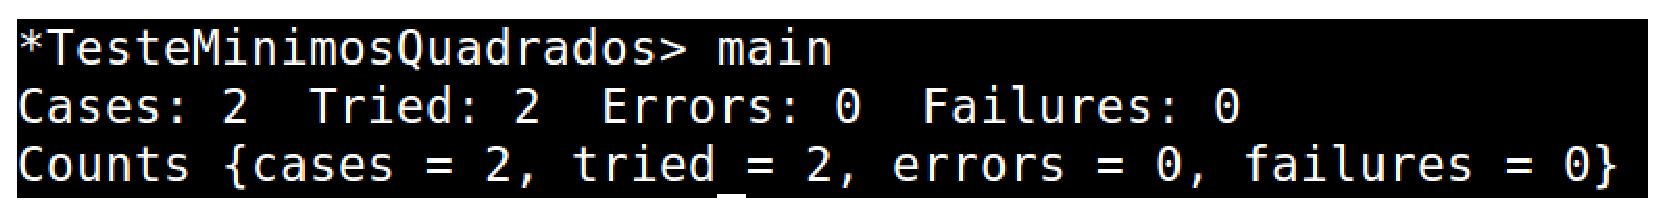
\includegraphics[width=0.9\textwidth]{figuras/TesteMinimosHaskell}
\caption{Resultado da Suíte de Teste do Método Mímimos Quadrados}
\label{TesteMinimosHaskell}
\end{figure}

Os códigos referentes aos testes unitários em linguagem Haskell encontram-se no apêndice F.

\subsection{Componente Estruturado}
\subsection{Componente Lógico}
Foi utilizada a ferramenta Swi-prolog para realização dos testes unitários na linguagem prolog. Não foi possível obter a cobertura de código fonte da linguagem prolog utilizando a ferramenta Swi-prolog (os testes ficaram com cobertura fixa em 4.5). Entretanto, os testes foram realizados com sucesso, conforme pode ser visualizado nas Figuras \ref{prologTeste1} e \ref{prologTeste2}. 

\begin{figure}[H]
\centering
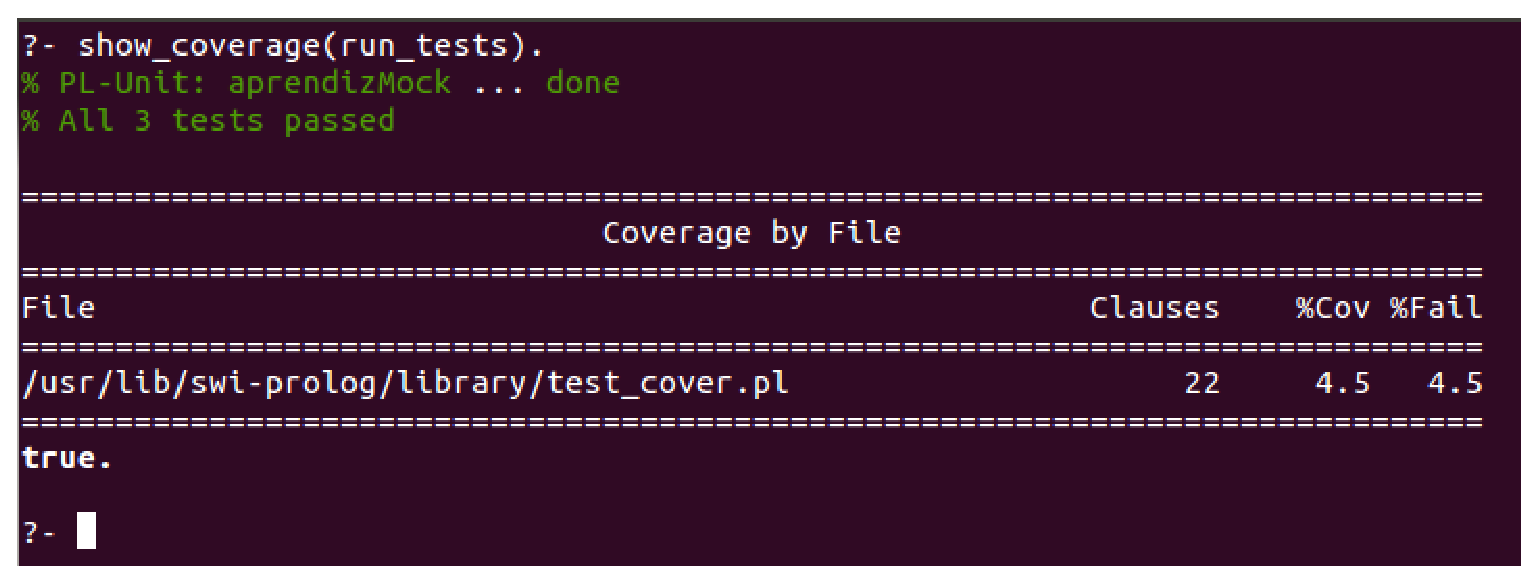
\includegraphics[width=0.9\textwidth]{figuras/prologTeste1}
\caption{Suíte de teste da base aprendiz.pl}
\label{prologTeste1}
\end{figure}

\begin{figure}[H]
\centering
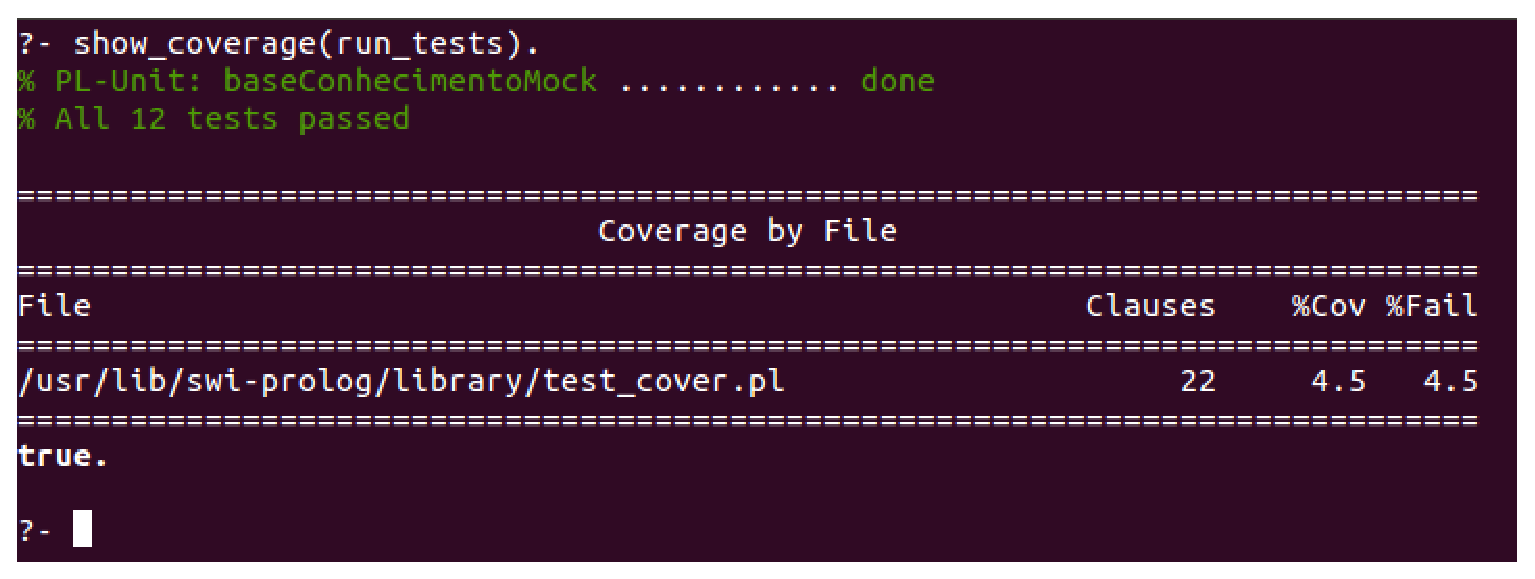
\includegraphics[width=0.9\textwidth]{figuras/prologTeste2}
\caption{Suíte de teste da base de conhecimento}
\label{prologTeste2}
\end{figure}

Os códigos referentes aos testes unitários em linguagem Prolog encontram-se no apêndice H.

\subsection{Componente Multiagentes}
Foram utilizados os frameworks Junit e Easy-mock para realização dos testes unitários na linguagem Java. Para obter a cobertura de código fonte, foi utilizada a ferramenta Eclemma. Obteve-se uma cobertura de código fonte de 84.8\% nos testes unitários, conforme pode ser visualizado na Figura \ref{eclemmaSMA}. 

\begin{figure}[H]
\centering
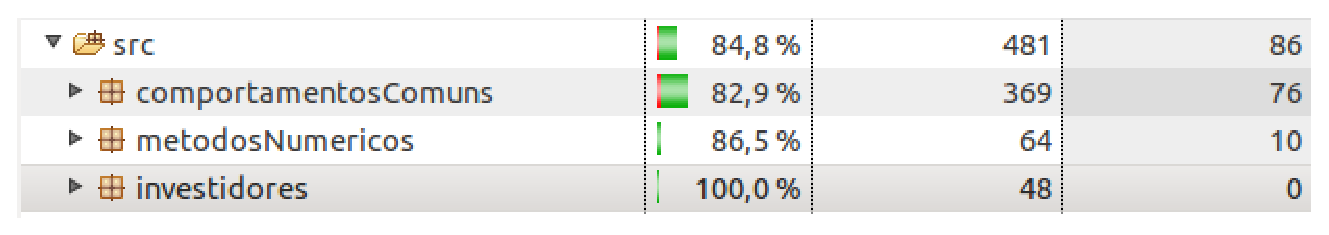
\includegraphics[width=0.9\textwidth]{figuras/eclemmaSMA}
\caption{Cobertura de Código dos pacotes do Componente Multiagentes}
\label{eclemmaSMA}
\end{figure}

O comportamento dos agentes são executados através dos métodos actions e muitos  comportamentos precisavam de um tempo de até 6 (seis) segundos para serem executados. Devido a isso, os testes unitários quebraram, pois nenhum comportamento era executado a tempo. Para tentar solucionar esse problema, foram colocados delays para que desse tempo dos agentes se comunicarem. A execução dos testes demorou mais de 18 (dezoito) segundos conforme pode ser visualizado no  canto superior esquerdo da Figura \ref{eclemmaTodasClasses}. Apesar de todos os testes passarem pelo Junit e o Easy-mock com os delays, a ferramenta Eclemma não pegava a cobertura de código dos métodos actions e devido a isso esses métodos foram ignorados no percentual de cobertura de código fonte.

\begin{figure}[H]
\centering
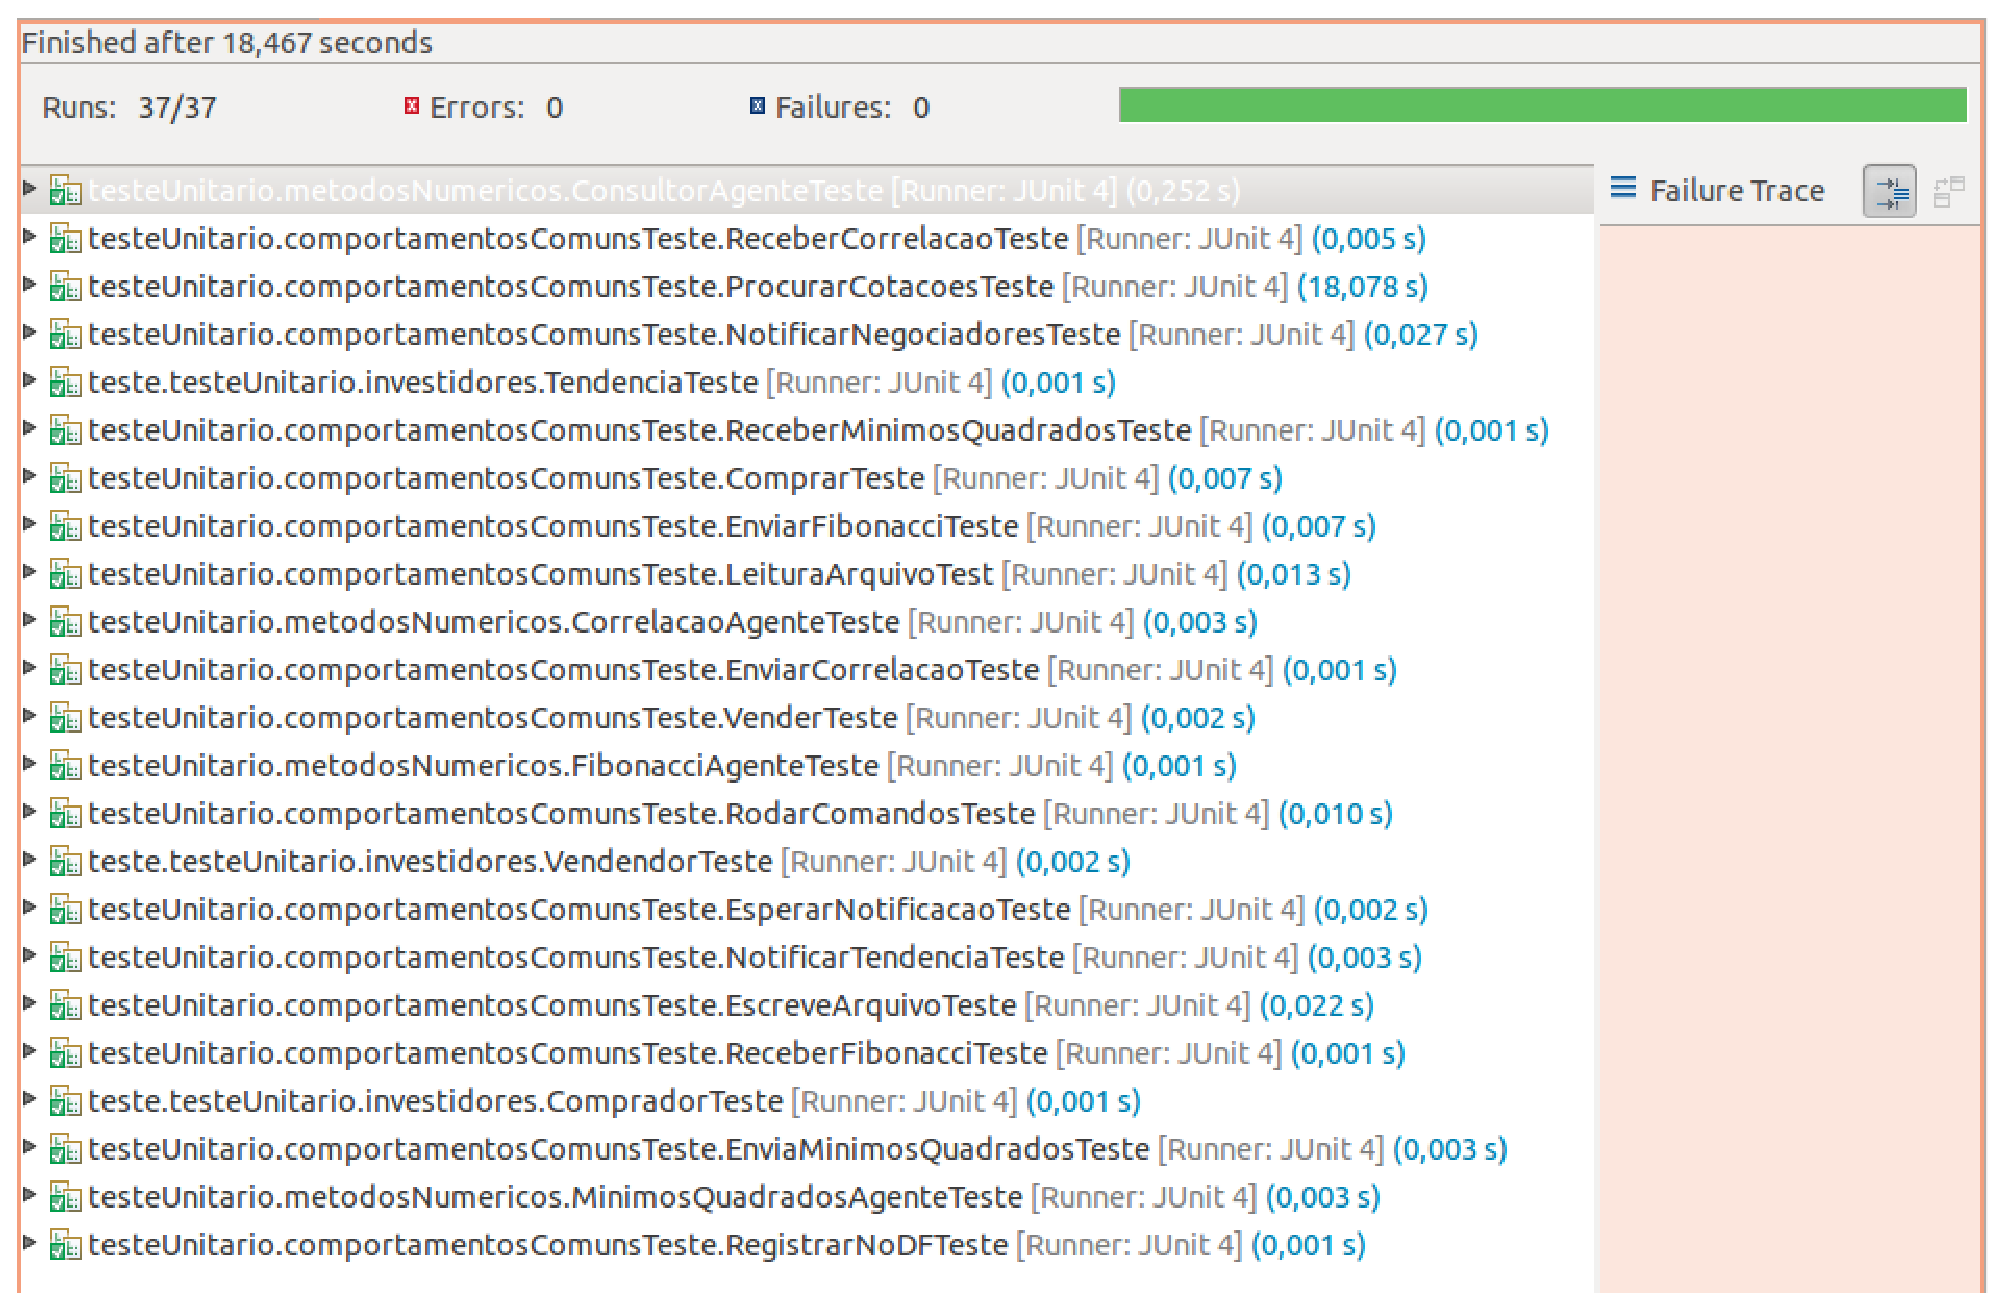
\includegraphics[width=0.9\textwidth]{figuras/eclemmaTodasClasses}
\caption{Suite de teste do Componente Multiagentes}
\label{eclemmaTodasClasses}
\end{figure}

As classes de teste mais significativas encontram-se no apêndice I.